In this lab, a simple brute-force attack program written in C was used to crack a hashed account password.

\section{Linux password storage}\label{sec:linux-password-storage}
Linux systems store user account details across two files, $/etc/passwd$ and $/etc/shadow$.
I learned information about this from
\href{https://www.cyberciti.biz/faq/understanding-etcpasswd-file-format/}{this site}~\autocite{accStorage},
which states that the public unencrypted ASCII file $/etc/passwd$ contains a line for each user on the system,
with publicly accessible information such as username, user ID and group ID, whereas the encrypted $/etc/shadow$
file contains the encrypted passwords of users on the system.

\begin{figure}[H]
    \centering
    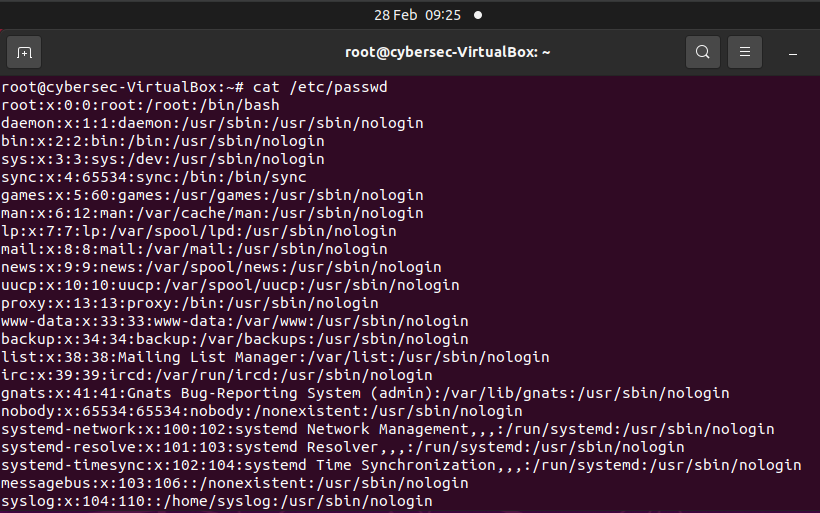
\includegraphics[width=.9\linewidth]{lab6/1}
    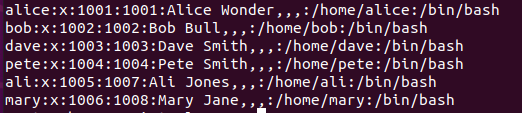
\includegraphics[width=.9\linewidth]{lab6/1b}
    \caption{Some of the contents of /etc/passwd, with the created users from earlier labs.}
    \label{fig:etcpasswd}
\end{figure}

\begin{figure}[H]
    \centering
    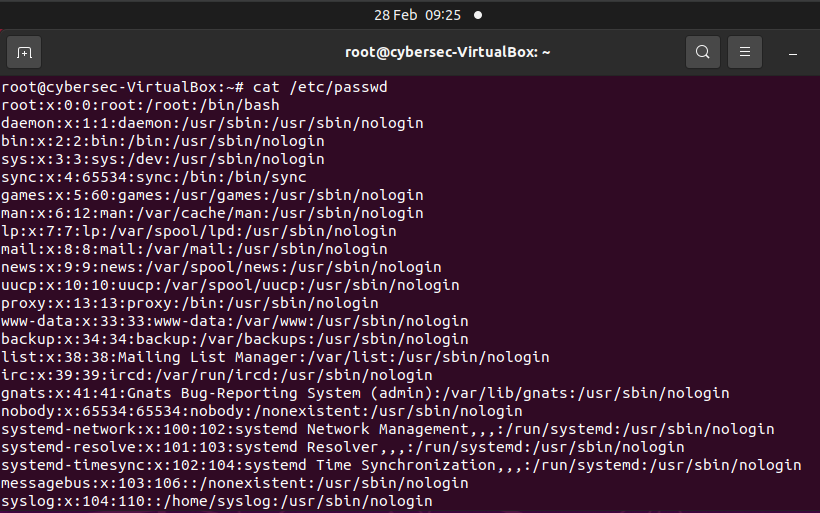
\includegraphics[width=.9\linewidth]{lab6/1}
    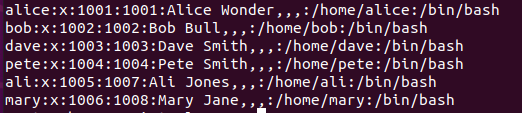
\includegraphics[width=.9\linewidth]{lab6/1b}
    \caption{Some of the contents of /etc/shadow, with the created users from earlier labs.}
    \label{fig:etcshadow}
\end{figure}



%\begin{itemize}
%    \item Username
%    \item Password - This doesn't store the actual password, which is located in $/etc/shadow$, but rather
%          an "x", indicative of if their encrypted and salted password is in the shadow file.
%    \item User ID
%    \item Primary group ID
%    \item User ID info - Comments such as their full name.
%    \item Home directory
%    \item The user's shell
%\end{itemize}



\section{crack.c}\label{sec:crack.c}
The provided code in crack.c is a small program that cracks passwords against the builtin Ubuntu dictionary,
located in $/usr/share/dict/words$.

\subsection{Importing and compilation}\label{subsec:importing-and-compilation}
First, this code must be ported into the Ubuntu VM using "nano crack.c", and pasting the code from Moodle
into the file.

\begin{figure}[H]
    \centering
    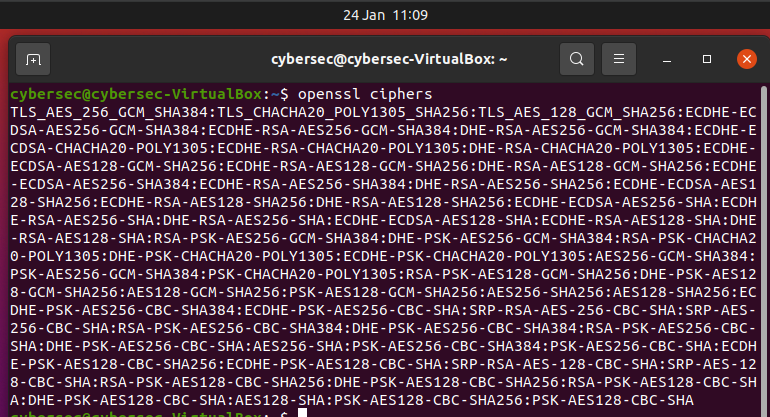
\includegraphics[width=.9\linewidth]{lab6/3}
    \caption{Porting crack.c into the VM.}
    \label{fig:nanoCrackC}
\end{figure}

Because C code can't be natively run, it must first be compiled.
This creates an executable called 'crack'.

\begin{figure}[H]
    \centering
    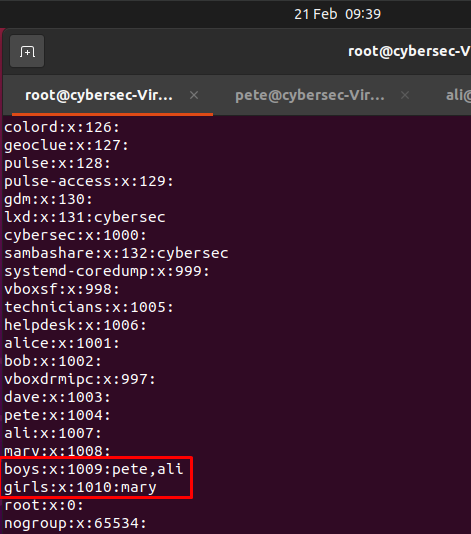
\includegraphics[width=.9\linewidth]{lab6/3b}
    \caption{Compiling crack.c.}
    \label{fig:compile}
\end{figure}

The '-lcrypt' argument supplies the Linux crypt library when compiling, allowing the crypt() function
to be used more securely.

\subsection{Creating a test user}\label{subsec:creating-a-test-user}
To use the program, it will be necessary to create a new user, whose password can be found in the dictionary.
For this, the user 'fred' will be created, and his password will be 'peach'.
We can see if 'peach' appears in the dictionary, as well as the overall dictionary word count.

\begin{figure}[H]
    \centering
    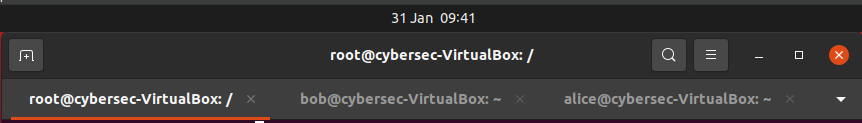
\includegraphics[width=.9\linewidth]{lab6/4}
    \caption{Checking the dictionary for the word 'peach', which is the 71496th entry.}
    \label{fig:checkDict}
\end{figure}

\begin{figure}[H]
    \centering
    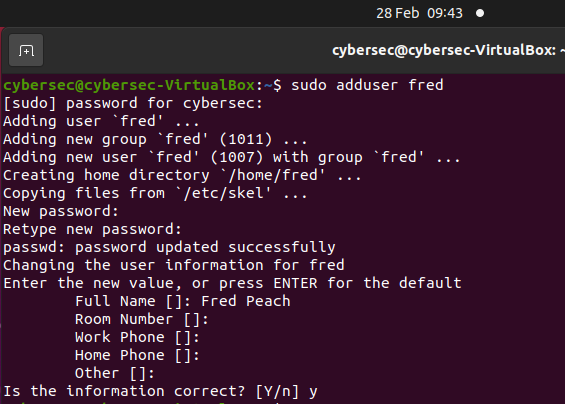
\includegraphics[width=.6\linewidth]{lab6/4b}
    \caption{Creating the 'fred' user, with the password 'peach'.}
    \label{fig:createFred}
\end{figure}

It will then be necessary to get the hashed version of Fred's password, which can be done using
"cat /etc/shadow | grep fred | awk -F: '\{ print \$2 \}'.
This command will read the shadow file, selecting the row starting with 'fred'.
Then, it will extract his hash by selecting the second column.

\begin{figure}[H]
    \centering
    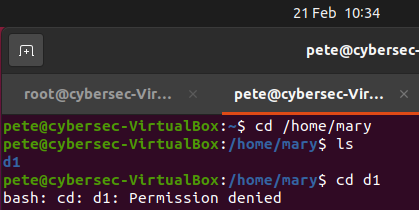
\includegraphics[width=.9\linewidth]{lab6/5}
    \caption{Viewing fred's hashed password.}
    \label{fig:viewFredHash}
\end{figure}

\subsection{Cracking the password}\label{subsec:cracking-the-password}
The program takes two arguments, with the first being the salt used on the password and the
second being the entire hashed password.
It requires the salt as an argument because it will apply the salt to each password it checks.
As seen in Figure \ref{fig:viewFredHash}, Fred's entire hashed password is

\begin{verbatim}
$6$5vbOyjaMeVhIrG5x$WUkun/BiYW0Hcw.zX6m1K2Y7zQR0tVdLMIKDjK0rIDQmiNQfsZa
52n.qUo.x1eut6zoJzg3Sx0RJAavLZO2TN.
\end{verbatim}

We can figure out the salt used on this password by looking at how it starts.
The first 20 characters of this password are the salt, noticeable by how they are between two dollar signs.
This can be supplied as the first argument for the compiled crack program, and the second argument would be the
entire password, including the salt as well.
Ultimately, this forms the following command:

\begin{verbatim}
./crack '$6$5vbOyjaMeVhIrG5x$'
'$6$5vbOyjaMeVhIrG5x$WUkun/BiYW0Hcw.zX6m1K2Y7zQR0tVdLMIKDjK0rIDQmiNQfsZa
52n.qUo.x1eut6zoJzg3Sx0RJAavLZO2TN.'
\end{verbatim}

It is imperative to use \textbf{quotation} marks rather than speech marks, as Linux will otherwise incorrectly
interpret the arguments given due to there being dollar signs in the hash, meaning that the crack will be
unsuccessful.

\begin{figure}[H]
    \centering
    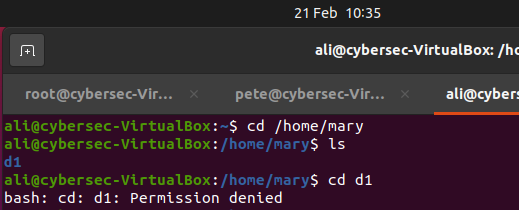
\includegraphics[width=\linewidth]{lab6/6}
    \caption{Entering the command.}
    \label{fig:cracking}
\end{figure}

\begin{figure}[H]
    \centering
    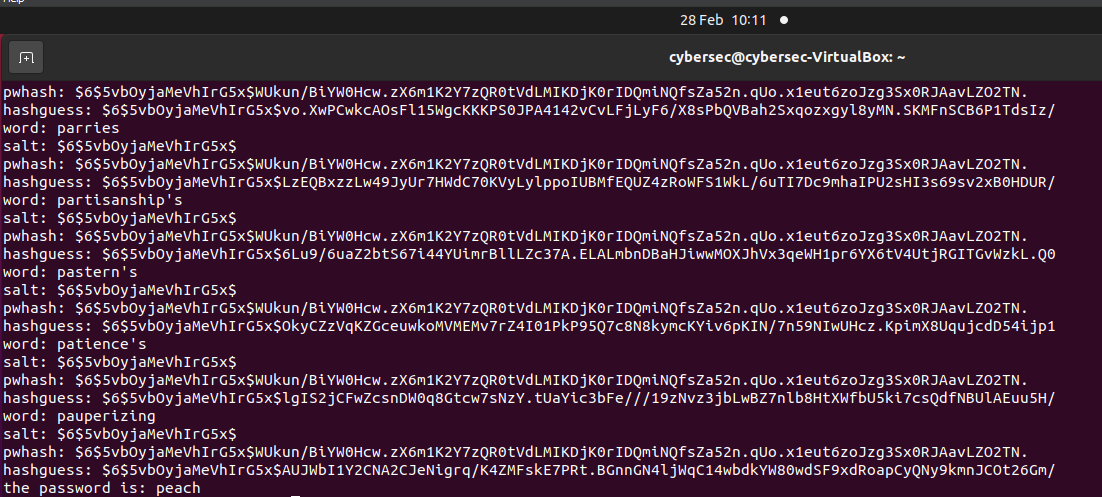
\includegraphics[width=.9\linewidth]{lab6/6b}
    \caption{The hashed password is revealed as 'peach'.}
    \label{fig:cracked}
\end{figure}

Note the differing timestamps, showing how this took around 3 minutes to execute, even on a 10-core
Intel i5-12600k.
This is because the word 'peach' occurs so late in the dictionary as seen in Figure \ref{fig:checkDict}.


